\documentclass[a4paper]{article}

%================================================================================================================================
%
% Packages
%
%================================================================================================================================

\usepackage[T1]{fontenc} 	% pour caractères accentués
\usepackage[utf8]{inputenc}  % encodage utf8
\usepackage[french]{babel}	% langue : français
\usepackage{fourier}			% caractères plus lisibles
\usepackage[dvipsnames]{xcolor} % couleurs
\usepackage{fancyhdr}		% réglage header footer
\usepackage{needspace}		% empêcher sauts de page mal placés
\usepackage{graphicx}		% pour inclure des graphiques
\usepackage{enumitem,cprotect}		% personnalise les listes d'items (nécessaire pour ol, al ...)
\usepackage{hyperref}		% Liens hypertexte
\usepackage{pstricks,pst-all,pst-node,pstricks-add,pst-math,pst-plot,pst-tree,pst-eucl} % pstricks
\usepackage[a4paper,includeheadfoot,top=2cm,left=3cm, bottom=2cm,right=3cm]{geometry} % marges etc.
\usepackage{comment}			% commentaires multilignes
\usepackage{amsmath,environ} % maths (matrices, etc.)
\usepackage{amssymb,makeidx}
\usepackage{bm}				% bold maths
\usepackage{tabularx}		% tableaux
\usepackage{colortbl}		% tableaux en couleur
\usepackage{fontawesome}		% Fontawesome
\usepackage{environ}			% environment with command
\usepackage{fp}				% calculs pour ps-tricks
\usepackage{multido}			% pour ps tricks
\usepackage[np]{numprint}	% formattage nombre
\usepackage{tikz,tkz-tab} 			% package principal TikZ
\usepackage{pgfplots}   % axes
\usepackage{mathrsfs}    % cursives
\usepackage{calc}			% calcul taille boites
\usepackage[scaled=0.875]{helvet} % font sans serif
\usepackage{svg} % svg
\usepackage{scrextend} % local margin
\usepackage{scratch} %scratch
\usepackage{multicol} % colonnes
%\usepackage{infix-RPN,pst-func} % formule en notation polanaise inversée
\usepackage{listings}

%================================================================================================================================
%
% Réglages de base
%
%================================================================================================================================

\lstset{
language=Python,   % R code
literate=
{á}{{\'a}}1
{à}{{\`a}}1
{ã}{{\~a}}1
{é}{{\'e}}1
{è}{{\`e}}1
{ê}{{\^e}}1
{í}{{\'i}}1
{ó}{{\'o}}1
{õ}{{\~o}}1
{ú}{{\'u}}1
{ü}{{\"u}}1
{ç}{{\c{c}}}1
{~}{{ }}1
}


\definecolor{codegreen}{rgb}{0,0.6,0}
\definecolor{codegray}{rgb}{0.5,0.5,0.5}
\definecolor{codepurple}{rgb}{0.58,0,0.82}
\definecolor{backcolour}{rgb}{0.95,0.95,0.92}

\lstdefinestyle{mystyle}{
    backgroundcolor=\color{backcolour},   
    commentstyle=\color{codegreen},
    keywordstyle=\color{magenta},
    numberstyle=\tiny\color{codegray},
    stringstyle=\color{codepurple},
    basicstyle=\ttfamily\footnotesize,
    breakatwhitespace=false,         
    breaklines=true,                 
    captionpos=b,                    
    keepspaces=true,                 
    numbers=left,                    
xleftmargin=2em,
framexleftmargin=2em,            
    showspaces=false,                
    showstringspaces=false,
    showtabs=false,                  
    tabsize=2,
    upquote=true
}

\lstset{style=mystyle}


\lstset{style=mystyle}
\newcommand{\imgdir}{C:/laragon/www/newmc/assets/imgsvg/}
\newcommand{\imgsvgdir}{C:/laragon/www/newmc/assets/imgsvg/}

\definecolor{mcgris}{RGB}{220, 220, 220}% ancien~; pour compatibilité
\definecolor{mcbleu}{RGB}{52, 152, 219}
\definecolor{mcvert}{RGB}{125, 194, 70}
\definecolor{mcmauve}{RGB}{154, 0, 215}
\definecolor{mcorange}{RGB}{255, 96, 0}
\definecolor{mcturquoise}{RGB}{0, 153, 153}
\definecolor{mcrouge}{RGB}{255, 0, 0}
\definecolor{mclightvert}{RGB}{205, 234, 190}

\definecolor{gris}{RGB}{220, 220, 220}
\definecolor{bleu}{RGB}{52, 152, 219}
\definecolor{vert}{RGB}{125, 194, 70}
\definecolor{mauve}{RGB}{154, 0, 215}
\definecolor{orange}{RGB}{255, 96, 0}
\definecolor{turquoise}{RGB}{0, 153, 153}
\definecolor{rouge}{RGB}{255, 0, 0}
\definecolor{lightvert}{RGB}{205, 234, 190}
\setitemize[0]{label=\color{lightvert}  $\bullet$}

\pagestyle{fancy}
\renewcommand{\headrulewidth}{0.2pt}
\fancyhead[L]{maths-cours.fr}
\fancyhead[R]{\thepage}
\renewcommand{\footrulewidth}{0.2pt}
\fancyfoot[C]{}

\newcolumntype{C}{>{\centering\arraybackslash}X}
\newcolumntype{s}{>{\hsize=.35\hsize\arraybackslash}X}

\setlength{\parindent}{0pt}		 
\setlength{\parskip}{3mm}
\setlength{\headheight}{1cm}

\def\ebook{ebook}
\def\book{book}
\def\web{web}
\def\type{web}

\newcommand{\vect}[1]{\overrightarrow{\,\mathstrut#1\,}}

\def\Oij{$\left(\text{O}~;~\vect{\imath},~\vect{\jmath}\right)$}
\def\Oijk{$\left(\text{O}~;~\vect{\imath},~\vect{\jmath},~\vect{k}\right)$}
\def\Ouv{$\left(\text{O}~;~\vect{u},~\vect{v}\right)$}

\hypersetup{breaklinks=true, colorlinks = true, linkcolor = OliveGreen, urlcolor = OliveGreen, citecolor = OliveGreen, pdfauthor={Didier BONNEL - https://www.maths-cours.fr} } % supprime les bordures autour des liens

\renewcommand{\arg}[0]{\text{arg}}

\everymath{\displaystyle}

%================================================================================================================================
%
% Macros - Commandes
%
%================================================================================================================================

\newcommand\meta[2]{    			% Utilisé pour créer le post HTML.
	\def\titre{titre}
	\def\url{url}
	\def\arg{#1}
	\ifx\titre\arg
		\newcommand\maintitle{#2}
		\fancyhead[L]{#2}
		{\Large\sffamily \MakeUppercase{#2}}
		\vspace{1mm}\textcolor{mcvert}{\hrule}
	\fi 
	\ifx\url\arg
		\fancyfoot[L]{\href{https://www.maths-cours.fr#2}{\black \footnotesize{https://www.maths-cours.fr#2}}}
	\fi 
}


\newcommand\TitreC[1]{    		% Titre centré
     \needspace{3\baselineskip}
     \begin{center}\textbf{#1}\end{center}
}

\newcommand\newpar{    		% paragraphe
     \par
}

\newcommand\nosp {    		% commande vide (pas d'espace)
}
\newcommand{\id}[1]{} %ignore

\newcommand\boite[2]{				% Boite simple sans titre
	\vspace{5mm}
	\setlength{\fboxrule}{0.2mm}
	\setlength{\fboxsep}{5mm}	
	\fcolorbox{#1}{#1!3}{\makebox[\linewidth-2\fboxrule-2\fboxsep]{
  		\begin{minipage}[t]{\linewidth-2\fboxrule-4\fboxsep}\setlength{\parskip}{3mm}
  			 #2
  		\end{minipage}
	}}
	\vspace{5mm}
}

\newcommand\CBox[4]{				% Boites
	\vspace{5mm}
	\setlength{\fboxrule}{0.2mm}
	\setlength{\fboxsep}{5mm}
	
	\fcolorbox{#1}{#1!3}{\makebox[\linewidth-2\fboxrule-2\fboxsep]{
		\begin{minipage}[t]{1cm}\setlength{\parskip}{3mm}
	  		\textcolor{#1}{\LARGE{#2}}    
 	 	\end{minipage}  
  		\begin{minipage}[t]{\linewidth-2\fboxrule-4\fboxsep}\setlength{\parskip}{3mm}
			\raisebox{1.2mm}{\normalsize\sffamily{\textcolor{#1}{#3}}}						
  			 #4
  		\end{minipage}
	}}
	\vspace{5mm}
}

\newcommand\cadre[3]{				% Boites convertible html
	\par
	\vspace{2mm}
	\setlength{\fboxrule}{0.1mm}
	\setlength{\fboxsep}{5mm}
	\fcolorbox{#1}{white}{\makebox[\linewidth-2\fboxrule-2\fboxsep]{
  		\begin{minipage}[t]{\linewidth-2\fboxrule-4\fboxsep}\setlength{\parskip}{3mm}
			\raisebox{-2.5mm}{\sffamily \small{\textcolor{#1}{\MakeUppercase{#2}}}}		
			\par		
  			 #3
 	 		\end{minipage}
	}}
		\vspace{2mm}
	\par
}

\newcommand\bloc[3]{				% Boites convertible html sans bordure
     \needspace{2\baselineskip}
     {\sffamily \small{\textcolor{#1}{\MakeUppercase{#2}}}}    
		\par		
  			 #3
		\par
}

\newcommand\CHelp[1]{
     \CBox{Plum}{\faInfoCircle}{À RETENIR}{#1}
}

\newcommand\CUp[1]{
     \CBox{NavyBlue}{\faThumbsOUp}{EN PRATIQUE}{#1}
}

\newcommand\CInfo[1]{
     \CBox{Sepia}{\faArrowCircleRight}{REMARQUE}{#1}
}

\newcommand\CRedac[1]{
     \CBox{PineGreen}{\faEdit}{BIEN R\'EDIGER}{#1}
}

\newcommand\CError[1]{
     \CBox{Red}{\faExclamationTriangle}{ATTENTION}{#1}
}

\newcommand\TitreExo[2]{
\needspace{4\baselineskip}
 {\sffamily\large EXERCICE #1\ (\emph{#2 points})}
\vspace{5mm}
}

\newcommand\img[2]{
          \includegraphics[width=#2\paperwidth]{\imgdir#1}
}

\newcommand\imgsvg[2]{
       \begin{center}   \includegraphics[width=#2\paperwidth]{\imgsvgdir#1} \end{center}
}


\newcommand\Lien[2]{
     \href{#1}{#2 \tiny \faExternalLink}
}
\newcommand\mcLien[2]{
     \href{https~://www.maths-cours.fr/#1}{#2 \tiny \faExternalLink}
}

\newcommand{\euro}{\eurologo{}}

%================================================================================================================================
%
% Macros - Environement
%
%================================================================================================================================

\newenvironment{tex}{ %
}
{%
}

\newenvironment{indente}{ %
	\setlength\parindent{10mm}
}

{
	\setlength\parindent{0mm}
}

\newenvironment{corrige}{%
     \needspace{3\baselineskip}
     \medskip
     \textbf{\textsc{Corrigé}}
     \medskip
}
{
}

\newenvironment{extern}{%
     \begin{center}
     }
     {
     \end{center}
}

\NewEnviron{code}{%
	\par
     \boite{gray}{\texttt{%
     \BODY
     }}
     \par
}

\newenvironment{vbloc}{% boite sans cadre empeche saut de page
     \begin{minipage}[t]{\linewidth}
     }
     {
     \end{minipage}
}
\NewEnviron{h2}{%
    \needspace{3\baselineskip}
    \vspace{0.6cm}
	\noindent \MakeUppercase{\sffamily \large \BODY}
	\vspace{1mm}\textcolor{mcgris}{\hrule}\vspace{0.4cm}
	\par
}{}

\NewEnviron{h3}{%
    \needspace{3\baselineskip}
	\vspace{5mm}
	\textsc{\BODY}
	\par
}

\NewEnviron{margeneg}{ %
\begin{addmargin}[-1cm]{0cm}
\BODY
\end{addmargin}
}

\NewEnviron{html}{%
}

\begin{document}
\meta{url}{/exercices/qcm-fonctions-bac-blanc-es-l-sujet-5-maths-cours-2018/}
\meta{pid}{10552}
\meta{titre}{QCM Fonctions - Bac blanc ES/L Sujet 5 - Maths-cours 2018}
\meta{type}{exercices}
%
\begin{h2}Exercice 2 (5 points)\end{h2}
\par
\emph{Pour chacune des cinq affirmations suivantes, indiquer si elle est vraie ou fausse en justifiant la réponse, soit à l'aide du graphique, soit par un calcul.\\ Il est attribué un point par réponse exacte correctement justifiée.\\ \textbf{Une réponse non justifiée n'est pas prise en compte.}}
\par
Soit la fonction $f$ définie sur l'intervalle $]0~;~5]$ par :
\par
\[f(x) =  \ln x - x + 3.  \]
\par
On a tracé ci-après la courbe représentative $\mathscr{C}_f$ de la fonction $f$, ainsi que $\mathscr{D}$, la tangente à la courbe $\mathscr{C}_f$ au point $A$ de coordonnées $(1~;~2)$.\\ Cette tangente est parallèle à l'axe des abscisses.
\par
On note respectivement $f'$ et $f''$ la dérivée et la dérivée seconde de la fonction $f$.
\par
\begin{center}
     \begin{extern}%width="500" alt="Courbe fonction et tangente"
          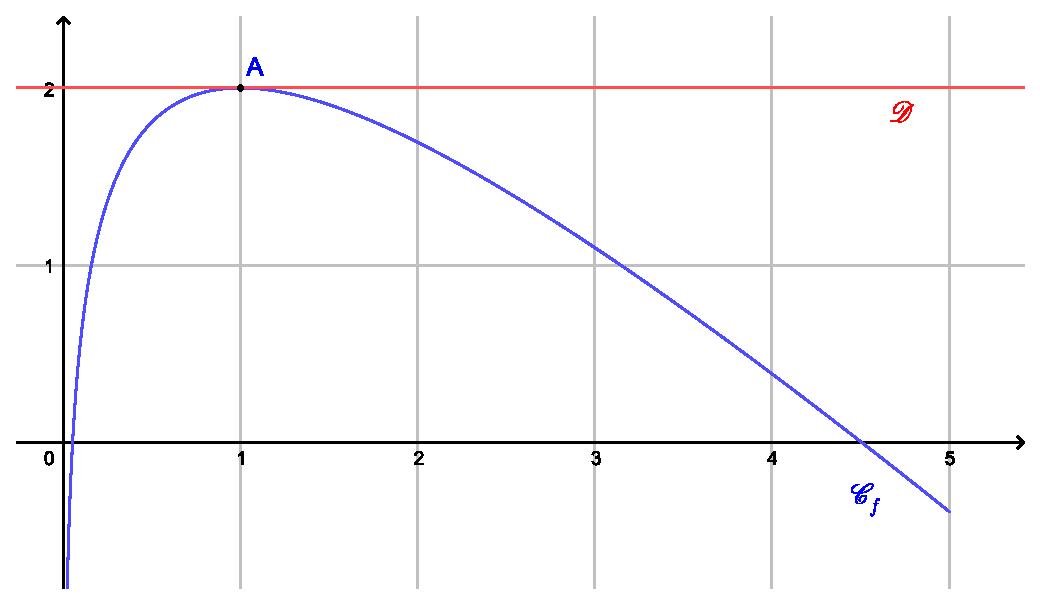
\includegraphics[width=0.9\textwidth]{images/BBESL-s5-2-1}% gbb 1 unite=3cm
     \end{extern}
\end{center}
\par
\begin{itemize}
     \item %1
     \textbf{Affirmation 1 :}\quad $f'(1)=0$.
     \item %2
     \textbf{Affirmation 2 :}\quad Pour tout réel $x$ de l'intervalle $]0~;~5]$, $f''(x)>0$.
     \item %3
     \textbf{Affirmation 3 :}\quad La courbe $\mathscr{C}_f$ possède un et un seul point d'inflexion.
     \item %4
     \textbf{Affirmation 4 :}\quad $1 \leqslant \displaystyle\int_{1}^{2}f(x)\text{d}x \leqslant 2$.
     \item %5
     \textbf{Affirmation 5 :}\quad La fonction $F$ définie sur l'intervalle $]0~;~5]$ par
     \par
     \[F(x) =  x\ln x - \dfrac{x^2}{2} + 3x  \]
     \par
     est une primitive de la fonction $f$ sur l'intervalle $]0~;~5]$.
     \par
\end{itemize}
\begin{corrige}
     \begin{itemize}
          \item %1
          \textbf{Affirmation 1 :}\quad $f'(1)=0$ : \textbf{VRAI}.
          \par
          \begin{itemize}
               \item
               \textbf{Méthode 1 : \`A l'aide du graphique}
               \par
               La tangente $\mathscr{D}$ à la courbe $\mathscr{C_f}$ au point $A$ est parallèle à l'axe des abscisses.
               \par
               $f'(1)$ est le coefficient directeur de $\mathscr{D}$ donc $f'(1)=0$.
               \par
               \cadre{rouge}{À retenir}{
                    Le \textbf{coefficient directeur de la tangente} à la courbe représentative de $f$ au point d'\textbf{abscisse} $\alpha$ est égal à $f'(\alpha)$.
                    \par
                    Si cette tangente est parallèle à l'axe des abscisses, $f'(\alpha) = 0$.
               }
               \item
               \textbf{Méthode 2 : Par le calcul}
               \par
               $f$ est dérivable sur l'intervalle $]0~;~5]$ comme somme de fonctions dérivables et :
               \par
               $f'(x)=\dfrac{1}{x}-1$.
               \par
               Par conséquent :
               \par
               $f'(1)=\dfrac{1}{1}-1=0$.
               \par
          \end{itemize}
          \item %2
          \textbf{Affirmation 2 :}\quad Pour tout réel $x$ de l'intervalle $]0~;~5]$, $f''(x)>0$ : \textbf{FAUX}.
          \par
          Pour tout réel $x$ de l'intervalle $]0~;~5]$, $f'(x)=\dfrac{1}{x}-1$ (voir question précédente). $f'$ est dérivable sur $]0~;~5]$ et :
          \par
          $f''(x)=-\dfrac{1}{x^2}.$
          \par
          $f''$ est strictement négative sur l'intervalle $]0~;~5]$, donc la proposition est fausse.
          \par
          \cadre{bleu}{Remarque}{
               Une autre possibilité consiste à dire que la courbe $\mathscr{C_f}$ est située \textbf{au-dessous} de ses tangentes donc que la fonction $f$ est \textbf{concave}.
               \par
               Cette méthode est toutefois moins rigoureuse ici, notamment, parce qu'au voisinage de 0, la courbe sort de l'image (par le bas) et qu'il est alors difficile de visualiser la position de la courbe et de ses tangentes...
          }
          \item %3
          \textbf{Affirmation 3 :}\quad La courbe $\mathscr{C}_f$ possède un et un seul point d'inflexion : \textbf{FAUX}.
          \par
          $f$ étant deux fois dérivable, la courbe $\mathscr{C_f}$ possède un point d'inflexion sur l'intervalle $]0~;~5]$ si et seulement $f''$ \textbf{s'annule et change de signe} en ce point. Or, d'après la question précédente, pour tout réel $x$ de l'intervalle $]0~;~5]$, $f''(x)<0$ donc la courbe $\mathscr{C_f}$ ne possède pas de point d'inflexion.
          \item %4
          \textbf{Affirmation 4 :}\quad $1 \leqslant \displaystyle\int_{1}^{2}f(x)\text{d}x \leqslant 2$ : \textbf{VRAI}.
          \par
          La fonction $f$ étant positive sur l'intervalle $]0~;~5]$, l'intégrale $\displaystyle\int_{1}^{2}f(x)\text{d}x$ est égale à l'aire, exprimée en unités d'aire, du domaine délimité par la courbe $\mathscr{C}_f$, l'axe des abscisses et les droites d'équations $x=1$ et $x=2$.
          \par
          Or, sur la figure, l'unité d'aire correspond à un carré du quadrillage. On voit donc facilement que :
          \[ 1 \leqslant \displaystyle\int_{1}^{2}f(x)\text{d}x \leqslant 2. \]
          \item %5
          \textbf{Affirmation 5 :}\quad La fonction $F$ définie sur l'intervalle $]0~;~5]$ par $F(x) =  x\ln x - \dfrac{x^2}{2} + 3x $ est une primitive de la fonction $f$ sur l'intervalle $]0~;~5]$ : \textbf{FAUX}.
          \par
          Pour tout réel $x$ strictement positif, posons :
          \[ u(x)=x \qquad \text{et} \qquad v(x)=\ln x. \]
          On en déduit :
          \[ u'(x)=1 \qquad \text{et} \qquad  v'(x)=\dfrac{1}{x}.\]
          Par conséquent :
          \par
          $(uv)'(x)=u'(x)v(x)+u(x)v'(x)=\ln x+x \times \dfrac{1}{x}=\ln x + 1$
          \par
          et :
          \par
          $F'(x)=\ln x + 1 - \dfrac{2x}{2} + 3 = \ln x - x + 4$.
          \par
          La fonction $F'$ est différente de la fonction $f$ donc $F$ \textbf{n'est pas} une primitive de la fonction $f$ sur l'intervalle $]0~;~5]$.
          \par
     \end{itemize}
\end{corrige}

\end{document}